\documentclass{article}

% if you need to pass options to natbib, use, e.g.:
%     \PassOptionsToPackage{numbers, compress}{natbib}
% before loading neurips_2019

% ready for submission
% \usepackage{neurips_2019}

% to compile a preprint version, e.g., for submission to arXiv, add add the
% [preprint] option:
%     \usepackage[preprint]{neurips_2019}

% to compile a camera-ready version, add the [final] option, e.g.:
     \usepackage[preprint]{neurips_2019}

% to avoid loading the natbib package, add option nonatbib:
%     \usepackage[nonatbib]{neurips_2019}

\usepackage[utf8]{inputenc} % allow utf-8 input
\usepackage[T1]{fontenc}    % use 8-bit T1 fonts
\usepackage{hyperref}       % hyperlinks
\usepackage{url}            % simple URL typesetting
\usepackage{booktabs}       % professional-quality tables
\usepackage{amsfonts}       % blackboard math symbols
\usepackage{nicefrac}       % compact symbols for 1/2, etc.
\usepackage{microtype}      % microtypography
\usepackage{graphicx}
\graphicspath{ {./} }
\title{Assignment 1}

% The \author macro works with any number of authors. There are two commands
% used to separate the names and addresses of multiple authors: \And and \AND.
%
% Using \And between authors leaves it to LaTeX to determine where to break the
% lines. Using \AND forces a line break at that point. So, if LaTeX puts 3 of 4
% authors names on the first line, and the last on the second line, try using
% \AND instead of \And before the third author name.

\author{%
Ankit Kumar \\
170121 \AND
   Chaitanya Pathare \\ 19111061\\ \AND
   Hemant Kumar \\ 170297\\ \AND
Rahul Ninaji Pakhare \\ 19111068 \\ \AND 
Raunak Kumar \\ 19111069\\
  % examples of more authors
  % \And
  % Coauthor \\
  % Affiliation \\
  % Address \\
  % \texttt{email} \\
  % \AND
  % Coauthor \\
  % Affiliation \\
  % Address \\
  % \texttt{email} \\
  % \And
  % Coauthor \\
  % Affiliation \\
  % Address \\
  % \texttt{email} \\
  % \And
  % Coauthor \\
  % Affiliation \\
  % Address \\
  % \texttt{email} \\
}

\begin{document}

\maketitle

\begin{abstract}
  Given The Squared SVM Solver we need to add dual constraint to it and define the Lagrangian function to it.And then eliminate the primal variables using first order optimality.Solve the problem with any 3 methods and plot it in graph
\end{abstract}

\section{Question}

Given equation 

=> $ argmin _{ w \epsilon R^d } \nicefrac{1}{2} \textbf{w} ^2  + C \Sigma _{i=1} ^n  ([ 1 - y^i < \textbf{w} ,  \textbf{x} ^i > ]_+)^2  \quad (P1) $

rewritten as new optimization problem

=> $ argmin _{ w \epsilon R^d } \nicefrac{1}{2}  \textbf{w} ^2 + C \Sigma _{i=1} ^n \xi  ^2  $ for all i $ \in [1,n] $

\[ s.t. \quad y^i <\textbf{w} ,  \textbf{x} ^i>  \geq 1 - \xi _i , \xi _i \geq 0 \quad for \quad all \quad i \in [1,n] \quad (P2)  \]

Introducing dual variable $ \alpha _i $ for each of the n constraints in (P2)

\[  L(w, \xi , \alpha ) =  \nicefrac{1}{2} \textbf{w}  ^2 + C \Sigma _{i=1} ^n \xi _i^2 + \Sigma _{i=1} ^n \alpha _i ( 1 - \xi _i -y^i< \textbf{w} ,  \textbf{x} ^i>) \quad, \alpha _i \geq 0  \qquad (P3) \]



\section{Question}

To get the dual problem  from the above equation (P3).
We have appended one extra dimension to our data i.e if X = $ \left[ \begin{array}{@{\,} ccccc @{\,}}
    x_{11}	& x_{12} & x_{13} & . & x_{1n}  \\
    x_{21} & \vdots & \vdots & \vdots  & x_{2n} \\
    \vdots & \vdots & \ddots & \ddots & \vdots \\
    \vdots & \vdots & \ddots & \ddots & \vdots \\
    x_{n1} & \vdots & \vdots & \vdots  & x_{nn} 
  \end{array} \right] $
 and then transformed  X $ \rightarrow X^0 = \left[ \begin{array}{@{\,} cccccc @{\,}}
    x_{11} & x_{12} & x_{13} &  .& x_{1n} & 1  \\
    x_{21} & . & . & . & x_{2n} & 1\\
    . & . & \ddots & \ddots & . & 1\\
    . & . & \ddots & \ddots& . & 1\\
    . & . & \ddots & \ddots& . & 1\\
    x_{n1} & . & . & .  & x_{nn} & 1\\
  \end{array} \right] $ so that w[d-1] =b , \{ d is dimension of each data point in $ X^0 $ \}
%\begin{equation}
%	 x&=10+y-z,\\ 
%	 y+z&=100,\\ 
%     z*y=z-12 
%\end{equation}



put $ \nicefrac{ \delta L }{ \delta \textbf{w} } = \textbf{0} and  \nicefrac{ \delta L }{ \delta \xi _i } = \textbf{0}  \quad for \quad all \quad i \in [1,n] $
\[ \nicefrac{ \delta L }{ \delta \textbf{w} } = \textbf{w} - \Sigma _{i=1} ^n \alpha _i \textbf{x} ^i = \textbf{0}  \]


\[ or \quad \textbf{w} = \Sigma _{i=1} ^n \alpha _i \textbf{x} ^i \]


 and

\[    \nicefrac{ \delta L }{ \delta \xi _i } =2C \xi _i  - \Sigma _{i=1} ^n \alpha _i = \textbf{0}  \]
\[ or \quad \xi _i = \nicefrac{1}{2C} \Sigma _{i=1} ^n \alpha _i  \]


Optimization problem comes down to 

\[ => \nicefrac{1}{2} \Sigma _{i=1} ^n \Sigma _{j=1} ^n ( \alpha _i \alpha _j y^i y^j< \textbf{x}^i \textbf{x}^j>) +  \nicefrac{1}{4C} \Sigma _{i=1} ^n  \alpha _i ^2 + \Sigma _{ i=1 } ^n \alpha_i - \nicefrac{1}{2C}\Sigma _{i=1} ^n  \alpha _i ^2 \]

 \[ - \Sigma _{i=1} ^n \Sigma _{j=1} ^n ( \alpha _i \alpha _j y^i y^j< \textbf{x}^i \textbf{x}^j>) \] 
 
% \Sigma _{i=1} ^n \Sigma _{j=1} ^n ( \alpha _i x^i y^i)(\alpha _j x^j y^j)) \]


 \[ \qquad => argmin(\Sigma _{i=1} ^n \alpha _i - \nicefrac{1}{4C} (\Sigma _{i=1} ^n  \alpha _i ^2) - \nicefrac{1}{2}\Sigma _{i=1} ^n \Sigma _{j=1} ^n ( \alpha _i \alpha _j y^i y^j< \textbf{x}^i \textbf{x}^j>)) \quad (D2) \]

\[ All \quad above \quad \textbf{w} \epsilon R ^{d+1} , \quad \textbf{x} \epsilon R ^{d+1} \]



\section{Question}



a. Mini Batch Stochastic Gradient descent on P1

Given,

	\[ P1 \quad f = \quad argmin _{ w \epsilon R^d } \nicefrac{1}{2} \textbf{w} ^2  + C \Sigma _{i=1} ^n  ([ 1 - y^i < \textbf{w} ,  \textbf{x} ^i > ]_+)^2   \]

now  get gradient for P1 

\[  \nabla f =  \textbf{w}  + 2 C \Sigma _{i=1} ^n  ([ 1 - y^i <\textbf{w} ,  \textbf{x} ^i> ]_+)(-y^i \textbf{x}^i) \]

\medskip

Note: $ [ 1 - y^i <\textbf{w} ,  \textbf{x} ^i> ]_+ = \{ ( 1 - y^i <\textbf{w} ,  \textbf{x} ^i> ) \quad if \quad y^i <\textbf{w} ,  \textbf{x} ^i> < 1 $ \\
\[ \quad \qquad  0 \quad if \quad y^i <\textbf{w} ,  \textbf{x} ^i> \geq 1 \} \] 

iterate till the time end for the X
\\

Do
\begin{verbatim}
  1.find gradient for each data point in the given Batch set B and step length eta  
  
  2.update w for these 
  \end{verbatim} 
   i.e,     $ \textbf{w} = \textbf{w} - \eta 2 C \Sigma _{i=x} ^{x+B}  ([ 1 - y^i <\textbf{w} ,  \textbf{x} ^i> ]_+)(-y^i \textbf{x}^i)$
 

Differengt cobination of (batch B) and step length $ \eta $ we tried are as follows,all works fine

\[
\begin{array}{@{\,} c|c @{\,}}
 B & \eta \\
  \hline
 10 & 0.01 \\
 100 & 0.05 \\
 1000 & 0.001 \\
\end{array}\] 


\medskip


b. Coordinate descent on P1


Given,

	\[ P1 \quad f = \quad argmin _{ w \epsilon R^d } \nicefrac{1}{2} \textbf{w} ^2  + C \Sigma _{i=1} ^n  ([ 1 - y^i < \textbf{w} ,  \textbf{x} ^i > ]_+)^2   \]

now  get gradient for P1 

\[  \nabla f =  \textbf{w}  + 2 C \Sigma _{i=1} ^n  ([ 1 - y^i <\textbf{w} ,  \textbf{x} ^i> ]_+)(-y^i \textbf{x}^i) \]



Note: $ [ 1 - y^i <\textbf{w} ,  \textbf{x} ^i> ]_+ = \{ ( 1 - y^i <\textbf{w} ,  \textbf{x} ^i> ) \quad if \quad y^i <\textbf{w} ,  \textbf{x} ^i> < 1 $ \\
\[ \quad \qquad  0 \quad if \quad y^i <\textbf{w} ,  \textbf{x} ^i> \geq 1 \} \] 


iterate till the time end for the X
\\

Do
\begin{verbatim}
  1.find gradient for each data point choosing the coordinate cyclically i,e j th= 1,2...d,1,2...d,...  
  
  2.update w for these 
  \end{verbatim} 
   i.e,     $ \textbf{w}  = \textbf{w} - \eta 2 C \Sigma _{i=1} ^{n}  ([ 1 - y^i <\textbf{w} ,  \textbf{x} ^i_{ j^th } > ]_+)(-y^i \textbf{x}^i _{ j^th } )$

Note :$ \eta $ value was choosen very small or else the curve diverges.

\medskip


c. Method used for  D2  maximization 

\[ D2  \qquad => argmax(\Sigma _{i=1} ^n \alpha _i - \nicefrac{1}{4C} (\Sigma _{i=1} ^n  \alpha _i ^2) - \nicefrac{1}{2}\Sigma _{i=1} ^n \Sigma _{j=1} ^n ( \alpha _i \alpha _j y^i y^j< \textbf{x}^i \textbf{x}^j>)) \]

concentrate on $ \alpha _i $

\[  argmax( \alpha _i - \nicefrac{1}{4C} (  \alpha _i ^2) -  (\Sigma _{i \neq j}   \alpha _j ^2) - \nicefrac{1}{2}( \alpha _i^2 ( \textbf{x} ^i )^2) - \alpha _iy^i\Sigma _{i \neq j}  (  \alpha _j  y^j< \textbf{x}^i \textbf{x}^j>)) \]


\[ Let \quad  x = \alpha _i , \quad q = ( \textbf{x} ^i ) ^2 , \quad p = y^i\Sigma _{i \neq j}  (  \alpha _j  y^j< \textbf{x}^i \textbf{x}^j>) , \quad r = (\Sigma _{i \neq j}   \alpha _j ^2) \]


\[  argmin(x^2( \nicefrac{1}{2} q + \nicefrac{1}{4C}) - x(1-p) + r ) \]

\[ Let \quad \nicefrac{ q ^0 }{2} = ( \nicefrac{q}{2} + \frac{1}{4C} ) \qquad    argmin( \nicefrac{ q ^0}{2} x^2 - x(1-p) + r ) \]




  minimum at $ x' = \nicefrac{ (1-p) }{ q^0 } $

  
  If $ x' \in [0,\infty] $ then $ x' $ is solution
  
   elseif $ x' < 0 $ solution is 0
   
    else solution is  $ \infty $.
  
  
Note: 
\[ p = y^i\Sigma _{i \neq j}  (  \alpha _j  y^j < x\textbf{x}^i \textbf{x}^j > ) \]

\[ = \textbf{w} ^T \textbf{x} ^i - \alpha _i  y^i q^0 \]

Algorithm minimize:

\[ intialize  \quad  \alpha  ^ T  =  \{ 0,0,........0 \}  _{ 1Xn } \quad \textbf{w} = \{ 0,0, .....0 \} _{1Xn} \]

\[ { \textbf{w} = \Sigma _{i=1} ^n \alpha _i y_i \textbf{x} ^i } \quad for \quad i \in [1,n] \]


\paragraph{Note:} We have appended one extra dimension to our data i.e if X = $ \left[ \begin{array}{@{\,} ccccc @{\,}}
    x_{11}	& x_{12} & x_{13} & . & x_{1n}  \\
    x_{21} & \vdots & \vdots & \vdots  & x_{2n} \\
    \vdots & \vdots & \ddots & \ddots & \vdots \\
    \vdots & \vdots & \ddots & \ddots & \vdots \\
    x_{n1} & \vdots & \vdots & \vdots  & x_{nn} 
  \end{array} \right] $
 and then transformed  X $ \rightarrow X^0 = \left[ \begin{array}{@{\,} cccccc @{\,}}
    x_{11} & x_{12} & x_{13} &  .& x_{1n} & 1  \\
    x_{21} & . & . & . & x_{2n} & 1\\
    . & . & \ddots & \ddots & . & 1\\
    . & . & \ddots & \ddots& . & 1\\
    . & . & \ddots & \ddots& . & 1\\
    x_{n1} & . & . & .  & x_{nn} & 1\\
  \end{array} \right] $ so that w[d-1] =b , \{ d is dimension of each data point in $ X^0 $ \}.Iterate till time does not end, for each data point in $ X^0 $ 
 
\medskip
   
 
  Do- 
     
     1. Calculate $ \alpha _i $ if $ \alpha _i \geq 0 $ then $ \alpha [i] = \alpha _i $
 
       else $ \alpha [i] = 0$
 
      2. Update w, $ \textbf{w} = \Sigma _{i=1} ^n \alpha _i y_i \textbf{x} ^i $
  
w will converge after sufficient number of iteration.   
   
   
   
\section{Question}
\paragraph{Hyperparameters used}
\paragraph{a.Mini Batch SGD on P1:}tried different values for Batch size from 10 to 1000 all gives similar results with $ \eta =$ 0.001 or 0.01.

\paragraph{b.Coordinate descent on P1:}here the step length need to be very small or else the curve diverges. We tried with step length 0.1 , 0.01 ,..and it kept on diverging.Thus fixed step length to a very small number 0.000001 that lead to convergence of the curve. 

\paragraph{c.Coordinate Maximization on D2:}No hyperparameter used.


\section{Question}
\paragraph{Figure:}Plot for convergence curves offered by those 3 method

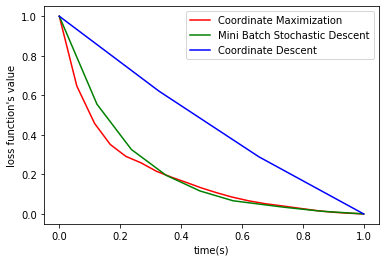
\includegraphics{converge}

Following graph was normalized using the minimum and maximum value for both the axis,as given below
\paragraph{a.Mini Batch SGD on P1:}

X axis (time): Min = 0.3228445053100586 Max = 3.0747430324554443

    Y axis (loss function value): Min = 5607.35 Max = 6252.87



\paragraph{b.Coordinate Descent on P1:}X axis (time): Min = 7.35390830039978 Max = 29.89153790473938

    Y axis (loss function value): Min = 13471.7  Max = 18036.3

    
    \paragraph{c.Coordinate Maximization on D2:}X axis (time): Min = 0.4362635612487793 Max = 9.31814169883728

    Y axis (loss function value): Min = 5236.12 Max = 9059.85



\section{Question}
Among the above three curves it is clear that Mini Batch Stochastic gradient descent gives the best convergence for the graph as seen in the plot.


\end{document}